\documentclass[11pt,a4paper]{article}

% ----- packages -----
\usepackage[T1]{fontenc}
\usepackage[utf8]{inputenc}
\usepackage{lmodern}
\usepackage[margin=2.4cm]{geometry}
\usepackage{microtype}
\usepackage{amsmath, amssymb, amsthm}
\usepackage{booktabs}
\usepackage{longtable}
\usepackage{array}
\usepackage{multirow}
\usepackage{xcolor}
\usepackage[table]{xcolor}
\usepackage[font=small,labelfont=bf]{caption}
\usepackage{listings}
\usepackage{hyperref}
\usepackage{tikz}
\usepackage{pgfplots}
\usepackage{pgfplotstable}
\pgfplotsset{compat=1.18}
\usetikzlibrary{positioning, arrows.meta, shapes.geometric, calc, patterns}

% ----- pgfplots setup -----
\definecolor{accentblue}{HTML}{1F4E79}
\definecolor{accentred}{HTML}{B22222}
\definecolor{accentgreen}{HTML}{2F6E2F}
\definecolor{cellref}{HTML}{F0F4F8}
\definecolor{cellbest}{HTML}{E8F4E8}

\hypersetup{
    colorlinks=true,
    linkcolor=accentblue,
    urlcolor=accentblue,
    citecolor=accentblue,
    pdftitle={WENO5 Mixed-Precision Benchmark on Consumer GPU},
    pdfauthor={FUNDAL precision benchmark}
}

\lstset{
    basicstyle=\ttfamily\footnotesize,
    columns=flexible,
    breaklines=true,
    breakatwhitespace=false,
    keepspaces=true,
    showstringspaces=false
}

% Pre-load CSV
\pgfplotstableread[col sep=comma, string type]{bench_ni32_numeric.csv}\benchdata

% ----- title -----
\title{
    \vspace{-1.5cm}
    \Large WENO5 Mixed-Precision Benchmark on Consumer NVIDIA GPU\\[0.3em]
    \large A 20-variant study of storage, compensation, parallelisation, and loop order\\[0.2em]
    \normalsize for the FUNDAL device-acceleration library
}
\author{FUNDAL precision benchmark}
\date{2026-05-19}

% ----- doc -----
\begin{document}
\maketitle
\vspace{-0.8em}

% ====================================================================
\begin{abstract}
\noindent We study, on a consumer-class NVIDIA RTX 4070 (Ada, \texttt{cc89}, with
\(\mathrm{FP64{:}FP32}\) ALU ratio \(1{:}64\)), the cost--benefit
landscape of mixed-precision arithmetic for a memory-bound
block-structured WENO5-JS stencil with forward-Euler (RK1) time
integration. Twenty kernel variants span a five-axis cross product:
storage precision (FP64, FP32, FP32-Dekker pair), rounding-error
compensation (Neumaier, Klein second-order, branchless FastTwoSum,
Graillat--Langlois compensated dot product, compensated Horner on
smoothness indicators), storage shape (\(U(b,i,j,k,c)\) vs
\(U(c,i,j,k,b)\)), parallelisation strategy
(\texttt{collapse(4)+vector} vs \texttt{collapse(5)}; Fortran-compliant
vs GPU ``biggest-stride-first'' lexical loop order), and
component-loop parallelism (\(c\) parallel or sequential, where the
latter mirrors the realistic-CFD constraint of nonlinear coupling
across conservative variables). All speedups are normalised to
\(\mathtt{V1'}\) --- FP64 with \(c\) sequential --- the honest
realistic-CFD baseline. We measure, over five independent trials at
production extents \((n_b, n_i, n_c, n_{\mathrm{steps}}) = (512, 32,
5, 100)\), median wall time, effective DRAM bandwidth, relative
\(L_2\) error vs FP64, and conservation drift. The headline
findings: (i)~the FP32 win survives the realistic-CFD constraint at
\(\sim 4.9\times\) over FP64 c-sequential and reaches \(\sim
123\times\) when \(c\) is parallel; (ii)~Dekker double-FP32 storage
reduces conservation drift to \(\mathrm{drMax} \approx 10^{-15}\),
within an order of magnitude of \(\varepsilon_{\mathrm{FP64}}\); (iii)
storage shape is irrelevant for pure FP64 kernels but matters
modestly (\(\sim 3\%\)) for compensated FP32-Dekker; (iv)
\texttt{!\$acc parallel loop collapse(N)} does \emph{not} abstract
away source lexical loop order on \texttt{nvfortran} 26.1 --- getting
it wrong costs \(\sim 10\times\). A complete catalogue of variants,
their mathematical and numerical models, error bounds, and
GPU-scheduling rationale is given.
\end{abstract}

% ====================================================================
\section{Goals}
\label{sec:goals}

The benchmark exists to answer four operational questions for FUNDAL,
in increasing order of specificity:

\begin{enumerate}
  \item \textbf{Is mixed-precision worth adopting on consumer NVIDIA
    GPUs?} The popular wisdom (``FP32 storage + FP64 compute'') is
    derived from CPU and datacenter-GPU experience where FP64
    throughput is comparable to FP32; on consumer Ada the
    \(\mathrm{FP64{:}FP32}\) ratio is \(1{:}64\), inverting the
    arithmetic regime. We test whether the textbook recipe survives
    the regime flip.
  \item \textbf{When mixed-precision \emph{is} adopted, which
    algorithm yields the best accuracy at minimum cost?} Five
    distinct compensated-arithmetic techniques --- spanning four
    decades of numerical-analysis literature, from Kahan--Babuska
    (1965) through Neumaier (1974), Dekker (1971), Klein (2006), and
    Graillat--Langlois (2008) --- are implemented and compared
    head-to-head on the same kernel.
  \item \textbf{Does GPU storage shape matter when the equations
    impose realistic constraints?} A real Euler / Navier--Stokes flux
    couples the \(n_c\) conservative variables nonlinearly, forbidding
    per-\(c\) parallelism. We test whether reorganising storage
    around the constraint (\(c\) leftmost / stride-1) recovers
    performance lost to the c-sequential loop.
  \item \textbf{Does the OpenACC \texttt{collapse(N)} clause abstract
    away source loop ordering?} CUDA-C convention suggests
    ``biggest-stride dimension first''; Fortran convention is
    ``stride-1 innermost''. Both cannot be correct on
    \texttt{nvfortran} with \texttt{collapse(N)}. We measure which
    rule the compiler actually follows.
\end{enumerate}

\section{Mathematical and numerical model}
\label{sec:math}

This section gives the precise formulas behind every kernel and
diagnostic.  Notation follows
\textit{Higham, Accuracy and Stability of Numerical Algorithms} (2nd
ed., SIAM 2002): \(\mathrm{fl}(x)\) is the correctly-rounded
floating-point value of a real expression \(x\); the unit roundoff is
\(u_{\mathrm{FP64}} = 2^{-53} \approx 1.11\times 10^{-16}\), \(u_{\mathrm{FP32}} = 2^{-24} \approx 5.96\times 10^{-8}\).

\subsection{Governing PDE and discretisation}
\label{sec:pde}

The benchmark integrates a 3-D scalar-by-scalar linear advection
system on each conservative component \(c\) of the state field
\(U_c(x,y,z,t)\):
\begin{equation}
\frac{\partial U_c}{\partial t} + \nabla \cdot \mathbf{F}(U_c) = 0,
\qquad \mathbf{F}(U_c) = (U_c, U_c, U_c).
\end{equation}
The triple-unit flux is a deliberately controlled probe (no shock
capturing, no pressure cancellation), so the only error sources are
the scheme and floating-point arithmetic.  Periodic BCs are imposed
per block via ghost-cell exchange ($n_g = 3$, since WENO5 requires a
7-point stencil).

Spatial discretisation is fifth-order Jiang--Shu finite-volume WENO:
\begin{equation}
\mathrm{rhs}_{ijk}^{(c)} = - \frac{1}{\Delta x}
\bigl(\hat F_{i+\tfrac12,jk}^{(c)} - \hat F_{i-\tfrac12,jk}^{(c)}\bigr)
- \frac{1}{\Delta y}\bigl(\cdots\bigr) - \frac{1}{\Delta z}\bigl(\cdots\bigr).
\end{equation}
Time integration is forward Euler with \(\Delta t = 10^{-3}\):
\(U^{n+1} = U^n + \Delta t \cdot \mathrm{rhs}^n\). RK1 is chosen
because it isolates per-step rounding (no inter-stage error
absorption masking compensation effects).

\subsection{WENO5-JS reconstruction}
\label{sec:weno5}

From a stencil \((v_{-2}, v_{-1}, v_0, v_{+1}, v_{+2})\), the left
state at \(i+\tfrac12\) is
\begin{equation}
\hat F^L_{i+\tfrac12} = \sum_{k=0}^{2} \omega_k\, p_k, \qquad
p_k = \tfrac{1}{6}\,\langle\text{3-point combination of stencil}\rangle.
\end{equation}
The nonlinear weights \(\omega_k\) are built from the smoothness
indicators (Jiang--Shu 1996):
\begin{equation}
\beta_k = \tfrac{13}{12}\,\Delta_2^{(k)}\!^2 + \tfrac{1}{4}\,\Delta_1^{(k)}\!^2,
\qquad
\alpha_k = \frac{d_k}{(\varepsilon + \beta_k)^2},
\qquad
\omega_k = \frac{\alpha_k}{\sum_j \alpha_j},
\end{equation}
with \(d = (0.1, 0.6, 0.3)\). The regularisation
\(\varepsilon\) is \(10^{-12}\) for FP64 and \(10^{-6}\) for FP32
(the latter chosen above the underflow boundary of \texttt{real32}).
Six WENO5 reconstructions are performed per cell per RK1 step (three
spatial directions \(\times\) two faces).

\subsection{Floating-point primitives}
\label{sec:fp-primitives}

All compensated variants share three IEEE-754 error-free transformations,
each operating entirely in working precision:
\begin{align}
\textbf{TwoSum}\quad s &= \mathrm{fl}(a + b), &
b' &= \mathrm{fl}(s - a), &
e &= \mathrm{fl}\bigl((a - \mathrm{fl}(s-b')) + (b - b')\bigr),
\end{align}
producing \((s, e)\) with \(a + b = s + e\) exactly in real
arithmetic, no precondition, 6 flops. \textbf{FastTwoSum} reduces to
3 flops assuming \(|a| \ge |b|\):
\begin{equation}
s = \mathrm{fl}(a + b), \qquad e = \mathrm{fl}(b - \mathrm{fl}(s - a)).
\end{equation}
\textbf{Veltkamp--Dekker TwoProd} (no FMA dependency) splits each
operand into 12-bit halves (splitter \(\sigma = 2^{12} + 1 = 4097\) for
FP32) and assembles a 17-flop exact product
\((h, \ell) = a \cdot b\).

\subsection{Per-variant compensation algorithms}
\label{sec:variants-algo}

\textbf{V3b --- KBN Neumaier.}  The RK1 update accumulates the
per-step rounding residual into a per-cell carry \(c\). With
\(y_n = \mathrm{fl}(\Delta t \cdot \mathrm{rhs}^n + c^{n-1})\):
\begin{equation}
t = \mathrm{fl}(U^n + y_n),
\quad
c^n = \begin{cases}
\mathrm{fl}\bigl((U^n - t) + y_n\bigr), & |U^n|\ge|y_n|\\
\mathrm{fl}\bigl((y_n - t) + U^n\bigr), & \text{otherwise}
\end{cases},
\quad
U^{n+1} = t.
\end{equation}
Per-step error \(\mathcal{O}(u)\) independent of step count
(Neumaier 1974).

\textbf{V3c --- Klein 2nd-order cascaded.}  Adds a second-level carry
\(c_2\) accumulating the rounding error of the \(c \mathrel{+}= \delta\)
update; \(U^{\mathrm{final}} = U + c + c_2\). Per-step error
\(\mathcal{O}(u^2)\) (Klein 2006). \emph{Empirically worse than V3b
in practice}: the first-level carry remains \(\mathcal{O}(u)\) and
\(c_2\) has nothing to catch at typical step counts.

\textbf{V3e --- Branchless FastTwoSum RK1.}  Drops the
\(|U|\ge|y|\) test that V3b carries; valid because
\(|U|=\mathcal{O}(1) \gg |\Delta t\cdot\mathrm{rhs}|=\mathcal{O}(10^{-3})\)
throughout the benchmark.  Same \(\mathcal{O}(u)\) per-step bound, no
warp divergence (Ogita--Rump 2005).

\textbf{V3d --- Graillat--Langlois compensated dot product.}
Replaces the 3-term reconstruction sum
\(\hat F = \omega_0 p_0 + \omega_1 p_1 + \omega_2 p_2\) with
TwoProd-and-TwoSum chains, accumulating rounding tails into a low
part: \(\hat F = t + (e_1 + e_2 + \ell_0 + \ell_1 + \ell_2)\). Error
\(u|\omega^\top p| + \mathrm{cond}(\omega^\top p)\,\gamma_3^2\,u^2\)
(Graillat--Langlois 2008).

\textbf{V3h --- Compensated Horner for \(\beta_k\).}  Each
\(\beta_k = K_1 d_1^2 + K_2 d_2^2\) is evaluated with TwoProd on each
square and TwoSum on the combination; \(\beta_k\) reassembled as
\(\beta_k^{(h)} + \beta_k^{(\ell)}\). Error bound
\(u|p(x)| + \mathrm{cond}(p,x)\,\gamma_{2n}^2\,u^2\)
(Graillat--Louvet 2007).

\textbf{V3f / V3g --- Dekker double-FP32 storage.}  State stored as a
pair \((U_h, U_\ell)\) with invariant
\(|U_\ell|\le\tfrac{1}{2}\mathrm{ulp}(U_h)\); reconstruction at each
load gives \(\sim\!48\)-bit effective mantissa. The update is a
two-stage TwoSum that absorbs the increment into the pair and
renormalises:
\begin{equation}
\begin{aligned}
\delta &= \mathrm{fl}(\Delta t\cdot\mathrm{rhs}), &
(s_1,e_1) &= \mathrm{TwoSum}(U_h, \delta), \\
\ell' &= \mathrm{fl}(U_\ell + e_1), &
(U_h^{n+1}, U_\ell^{n+1}) &= \mathrm{TwoSum}(s_1, \ell').
\end{aligned}
\end{equation}
The Dekker invariant is preserved, and the rounding residual of
\emph{every} arithmetic step is captured in the pair. V3g adds the
V3d compensated-dot reconstruction on top.

\subsection{Diagnostics}
\label{sec:diagnostics}

Per block \(b \in \{1,\dots,n_b\}\), we compute relative \(L_2\) error
\(\mathrm{err}_b\) and conservation drift \(\mathrm{drift}_b\):
\begin{equation}
\mathrm{err}_b =
\frac{\sqrt{\sum_{c,i,j,k} (U_b - U^{\mathrm{ref}}_b)^2}}
     {\sqrt{\sum_{c,i,j,k} (U^{\mathrm{ref}}_b)^2}},
\qquad
\mathrm{drift}_b =
\max_c \frac{|S(U^n_{b,c}) - S(U^0_{b,c})|}{\max(S(|U^0_{b,c}|), \tau)},
\end{equation}
where \(S(\cdot)\) is a pairwise (binary tree) summation operator
with error bound
\(\bigl|S_{\mathrm{pw}}(a) - \sum a_i\bigr| \le \lceil \log_2 n\rceil\,u\,\sum|a_i|\)
(Higham, Thm.~4.6). At \(N = n_i^3 = 32{\,}768\) cells per block, this
gives diagnostic error \(\le 15 u_{\mathrm{FP64}} \approx 1.7\times 10^{-15}\),
three orders of magnitude below the naive-sum bound and below the
\(\mathrm{drMax}\) signal we want to read for V1 and V3f-family
variants. Aggregated metrics
\(\mathrm{errMax} = \max_b \mathrm{err}_b\) etc.\ are reported.

\section{Variant catalogue}
\label{sec:catalogue}

Table~\ref{tab:variants} lists all 20 variants with their algorithmic
characteristics. Variants are grouped by precision regime and
parallelisation axis. The reference for the speedup column
throughout this report is \(\mathtt{V1'}\) (FP64 with c-loop
sequential), the honest realistic-CFD baseline.

{\footnotesize
\begin{longtable}{@{}p{1.0cm}p{2.2cm}p{2.5cm}p{2.4cm}p{6.5cm}@{}}
\caption{Variant catalogue.  ``shape A'' \(=\,U(b,i,j,k,c)\); ``shape B'' \(=\,U(c,i,j,k,b)\). ``order F'' \(=\,\)Fortran-compliant (stride-1 array dim lexically innermost in parallel set); ``order G'' \(=\,\)NVIDIA biggest-stride-first.} \label{tab:variants} \\
\toprule
\textbf{Tag} & \textbf{Precision} & \textbf{Storage} & \textbf{Parallelism} & \textbf{Algorithm / what it tests} \\
\midrule
\endfirsthead
\toprule
\textbf{Tag} & \textbf{Precision} & \textbf{Storage} & \textbf{Parallelism} & \textbf{Algorithm / what it tests} \\
\midrule
\endhead
V1     & FP64 throughout & shape A & c-par,~collapse(5)      & Production-grade reference; all FP32 errors are diffed against this run. \\
V1'    & FP64 throughout & shape A & c-seq,~collapse(4)+seq c & \textbf{Honest baseline for realistic CFD} (nonlinear coupling forbids per-c parallelism). REFERENCE for the universal speedup column. \\
V1B    & FP64 throughout & shape B & c-par,~collapse(5)      & Shape B counterpart of V1: tests storage shape effect for c-parallel FP64. \\
V1B'   & FP64 throughout & shape B & c-seq,~collapse(4)+seq c & Shape B counterpart of V1'. \\
V2     & FP32 store + FP64 compute (blanket) & shape A & c-par,~collapse(5) & The textbook ``mixed-precision middle path''. \\
V2b    & FP32 + FP64 \(\beta\) only & shape A & c-par,~collapse(5) & Surgical FP64 promotion of WENO5 smoothness indicators only. \\
V3     & FP32 throughout (naive) & shape A & c-par,~collapse(5) & FP32 baseline, no compensation. \\
V3b    & FP32 + Neumaier RK1 & shape A & c-par,~collapse(5)   & Kahan--Babuska--Neumaier compensated time integration. \\
V3c    & FP32 + Klein 2nd-order RK1 & shape A & c-par,~collapse(5) & Two cascaded carry arrays; \(\mathcal{O}(u^2)\) per step. \\
V3e    & FP32 + branchless FastTwoSum RK1 & shape A & c-par,~collapse(5) & Ogita--Rump unconditional Sum2; eliminates warp divergence. \\
V3d    & FP32 + compdot recon + Neumaier & shape A & c-par,~collapse(5) & Graillat--Langlois compensated dot on \(\hat F = \sum\omega_k p_k\). \\
V3h    & FP32 + comp Horner \(\beta\) + Neumaier & shape A & c-par,~collapse(5) & Compensated Horner on smoothness indicators. \\
V3f    & FP32-Dekker pair storage & shape A & c-par,~collapse(4)+inner vector & Double-FP32 \((U_h, U_\ell)\) with TwoSum update; \(\sim\!48\)-bit effective mantissa on every load. \\
V3g    & V3f + compdot recon & shape A & c-par,~collapse(4)+inner vector & Composition of V3f and V3d. \\
V3f'   & V3f with collapse(5) & shape A & c-par,~collapse(5)  & Tests collapse(5) vs collapse(4)+vector on the same Dekker kernel. \\
V3f''  & V3f with bad source loop order & shape A & c-par,~collapse(5) over (b,k,j,i,c) & Tests whether collapse(N) abstracts away source lexical order. \\
V3fA-F & FP32-Dekker, realistic CFD & shape A & c-seq, order F & Realistic constraint applied; stride-1 dim (b) lexically innermost. \\
V3fA-G & FP32-Dekker, realistic CFD & shape A & c-seq, order G & Realistic constraint; ``biggest stride first'' loop order. \\
V3fB-F & FP32-Dekker, realistic CFD & shape B & c-seq, order F & Shape B + order F; stride-1 dim (c) sequential, parallel-set stride-1 (i) lexically innermost. \\
V3fB-G & FP32-Dekker, realistic CFD & shape B & c-seq, order G & Shape B + order G. \\
\bottomrule
\end{longtable}
}

\section{Methodology}
\label{sec:method}

\paragraph{Hardware and toolchain.} NVIDIA RTX 4070 Ada
(\texttt{cc89}, \(12{,}282\)~MiB VRAM, \(\mathrm{FP64{:}FP32}\) ALU
ratio \(1{:}64\)); \texttt{nvhpc}~26.1 with \texttt{nvfortran -O2
-acc=gpu -gpu=cc89}. The second RTX 4070 in the system is left idle
to eliminate inter-card interference (\texttt{CUDA\_VISIBLE\_DEVICES=0}).

\paragraph{Problem extents.}
\((n_b, n_i, n_g, n_c, n_{\mathrm{steps}}) = (512, 32, 3, 5, 100)\).
Per FP64 array bytes \(= n_b\cdot(n_i+2n_g)^3\cdot n_c\cdot 8 \approx 1.07\)~GiB,
exceeding Ada's L2 cache and forcing honest HBM traffic. Peak VRAM
during the 20-variant run is \(\sim 5.3\)~GiB; the card has \(\sim
7\)~GiB headroom.

\paragraph{Timing protocol.}  Each variant runs \(n_{\mathrm{warm}} =
10\) untimed RK1 steps inside a structured \texttt{!\$acc data} region
to populate the device cache and dispatch the JIT module, then
\(n_{\mathrm{steps}} = 100\) timed steps. The timer is wall-clock
(\texttt{system\_clock}, not \texttt{cpu\_time}, which would report
near-zero on GPU offload), bracketed by \texttt{!\$acc wait} on both
ends to ensure asynchronous kernel completion before reading the
clock.

\paragraph{Statistics.}  Five independent program invocations of the
full 20-variant panel (each \(\approx 10\)~minutes wall time, total
\(\approx 50\)~minutes). Within each invocation all variants share
thermal state; across invocations the first \(\approx 1\)~s of each
variant absorbs JIT-module load. Median across the five trials is
reported; medians are robust to JIT-cache contention outliers (see
discussion in Sec.~\ref{sec:results}).

\paragraph{Reference and pairing.}  All speedups in this report use
\(\mathtt{V1'}\) (FP64 c-sequential, shape A) as the denominator:
\(\mathrm{speedup}_v = \mathrm{median}_{\text{trial}}
(t_{\mathtt{V1'}}/t_v)\).  Per-trial pairing eliminates between-trial
state variation from the comparison.

\section{Results}
\label{sec:results}

\subsection{Comprehensive measurement table}

Table~\ref{tab:results} reports the 5-trial measurements for every
variant. Median wall time and median bandwidth are reported with the
range (min--max across trials) for stability assessment; numerical
quality is given as median \(\mathrm{errMax}\) (relative \(L_2\) over
worst block) and median \(\mathrm{drMax}\) (conservation drift,
worst block, normalised by \(L_1\) norm of initial state).

{\scriptsize
\begin{longtable}{@{}lp{2.3cm}p{2.2cm}rrrrr@{}}
\caption{Five-trial measurement at \(n_i = 32\). Reference =
\(\mathtt{V1'}\) (FP64 c-sequential, shape A). Speedup = median of
per-trial ratios \(t_{\mathtt{V1'}}/t_v\). Conservation drift
\(\mathrm{drMax}\) for FP64 variants reaches
\(\varepsilon_{\mathrm{FP64}} \approx 1.76\!\times\!10^{-16}\), the
machine floor.} \label{tab:results} \\
\toprule
\textbf{Tag} & \textbf{Storage} & \textbf{c-mode} & \textbf{med t [s]} & \textbf{BW [GB/s]} & \textbf{vs V1'} & \textbf{errMax} & \textbf{drMax} \\
\midrule
\endfirsthead
\toprule
\textbf{Tag} & \textbf{Storage} & \textbf{c-mode} & \textbf{med t [s]} & \textbf{BW [GB/s]} & \textbf{vs V1'} & \textbf{errMax} & \textbf{drMax} \\
\midrule
\endhead
\texttt{V1} & \scriptsize\texttt{(b,i,j,k,c)} & c-parallel & 28.50 & 15.8 & 7.24\(\times\) & \(0\) & \(1.76{\times}10^{-16}\) \\
\textbf{\texttt{V1'}} & \scriptsize\textbf{\texttt{(b,i,j,k,c)}} & \textbf{c-sequential} & \textbf{206.65} & \textbf{2.2} & \textbf{1.00\(\times\) (REF)} & \textbf{\(0\)} & \textbf{\(1.76{\times}10^{-16}\)} \\
\texttt{V1B} & \scriptsize\texttt{(c,i,j,k,b)} & c-parallel & 28.43 & 15.8 & 7.28\(\times\) & \(0\) & \(1.76{\times}10^{-16}\) \\
\texttt{V1B'} & \scriptsize\texttt{(c,i,j,k,b)} & c-sequential & 206.63 & 2.2 & 0.99\(\times\) & \(0\) & \(1.76{\times}10^{-16}\) \\
\texttt{V2} & \scriptsize\texttt{(b,i,j,k,c)} & c-parallel & 28.93 & 7.8 & 7.14\(\times\) & \(1.11{\times}10^{-6}\) & \(5.20{\times}10^{-8}\) \\
\texttt{V3} & \scriptsize\texttt{(b,i,j,k,c)} & c-parallel & 1.67 & 134.6 & 122.79\(\times\) & \(1.11{\times}10^{-6}\) & \(5.06{\times}10^{-8}\) \\
\texttt{V2b} & \scriptsize\texttt{(b,i,j,k,c)} & c-parallel & 23.28 & 9.7 & 9.01\(\times\) & \(1.11{\times}10^{-6}\) & \(5.21{\times}10^{-8}\) \\
\texttt{V3b} & \scriptsize\texttt{(b,i,j,k,c)} & c-parallel & 1.72 & 130.9 & 121.19\(\times\) & \(7.47{\times}10^{-8}\) & \(2.18{\times}10^{-9}\) \\
\texttt{V3c} & \scriptsize\texttt{(b,i,j,k,c)} & c-parallel & 1.86 & 121.1 & 110.65\(\times\) & \(1.68{\times}10^{-7}\) & \(2.66{\times}10^{-9}\) \\
\texttt{V3e} & \scriptsize\texttt{(b,i,j,k,c)} & c-parallel & 1.84 & 122.3 & 112.28\(\times\) & \(7.47{\times}10^{-8}\) & \(2.18{\times}10^{-9}\) \\
\texttt{V3d} & \scriptsize\texttt{(b,i,j,k,c)} & c-parallel & 1.97 & 114.0 & 104.84\(\times\) & \(7.47{\times}10^{-8}\) & \(2.23{\times}10^{-9}\) \\
\texttt{V3h} & \scriptsize\texttt{(b,i,j,k,c)} & c-parallel & 2.15 & 104.4 & 95.14\(\times\) & \(7.47{\times}10^{-8}\) & \(2.18{\times}10^{-9}\) \\
\texttt{V3f} & \scriptsize\texttt{(b,i,j,k,c)} & c-parallel & 2.64 & 170.0 & 77.33\(\times\) & \(6.46{\times}10^{-8}\) & \(1.41{\times}10^{-15}\) \\
\texttt{V3g} & \scriptsize\texttt{(b,i,j,k,c)} & c-parallel & 2.82 & 159.3 & 73.18\(\times\) & \(6.46{\times}10^{-8}\) & \(1.04{\times}10^{-15}\) \\
\texttt{V3f'} & \scriptsize\texttt{(b,i,j,k,c)} & c-parallel & 2.39 & 188.4 & 85.69\(\times\) & \(6.46{\times}10^{-8}\) & \(1.41{\times}10^{-15}\) \\
\texttt{V3f"} & \scriptsize\texttt{(b,i,j,k,c)} & c-parallel & 23.54 & 19.1 & 8.69\(\times\) & \(6.46{\times}10^{-8}\) & \(1.41{\times}10^{-15}\) \\
\texttt{V3fA-F} & \scriptsize\texttt{(b,i,j,k,c)} & c-sequential & 43.65 & 10.3 & 4.74\(\times\) & \(6.46{\times}10^{-8}\) & \(1.41{\times}10^{-15}\) \\
\texttt{V3fA-G} & \scriptsize\texttt{(b,i,j,k,c)} & c-sequential & 44.99 & 10.0 & 4.54\(\times\) & \(6.46{\times}10^{-8}\) & \(1.41{\times}10^{-15}\) \\
\texttt{V3fB-F} & \scriptsize\texttt{(c,i,j,k,b)} & c-sequential & 42.35 & 10.6 & 4.89\(\times\) & \(6.46{\times}10^{-8}\) & \(1.41{\times}10^{-15}\) \\
\texttt{V3fB-G} & \scriptsize\texttt{(c,i,j,k,b)} & c-sequential & 46.03 & 9.8 & 4.55\(\times\) & \(6.46{\times}10^{-8}\) & \(1.41{\times}10^{-15}\) \\
\bottomrule
\end{longtable}
}

\subsection{Speedup chart}

Figure~\ref{fig:speedup} plots the median speedup of every variant
relative to V1' on a logarithmic scale. The three production regimes
are clearly separated: (i)~the V1/V2/V2b cluster at \(\sim
7\!-\!9\times\) (FP64 with c-parallelism, with or without FP32
storage overlay); (ii)~the FP32-with-compensation cluster at
\(\sim 80\!-\!120\times\) (V3, V3b, V3c, V3e, V3d, V3h, V3f, V3g,
V3f'); (iii)~the realistic-CFD c-sequential cluster at
\(\sim 4.5\!-\!4.9\times\) (V3fA-F, V3fA-G, V3fB-F, V3fB-G).
V3f'' (bad loop order) sits anomalously low at \(\sim 8.7\times\),
illustrating the cost of getting OpenACC source loop order wrong.

\begin{figure}[!htb]
\centering
\begin{tikzpicture}
\begin{axis}[
    width=0.97\textwidth, height=10cm,
    ybar, bar width=10pt,
    ymode=log, log basis y=10,
    ymin=0.7, ymax=300,
    ylabel={Speedup vs V1' (FP64 c-sequential, log scale)},
    xlabel={Variant},
    xtick=data,
    xticklabels from table={\benchdata}{short},
    xticklabel style={rotate=55, anchor=north east, font=\footnotesize},
    nodes near coords,
    nodes near coords style={font=\tiny, rotate=90, anchor=west, /pgf/number format/.cd, fixed, precision=1, fixed zerofill=false},
    grid=major, grid style={dashed, gray!30},
    axis line style={->, thick},
    every axis plot/.append style={fill=accentblue!70, draw=accentblue, line width=0.2pt},
]
\addplot table[x expr=\coordindex, y=med_spd, col sep=comma] {bench_ni32_numeric.csv};
\draw[dashed, accentred, thick] (axis cs:-0.5,1) -- (axis cs:19.5,1)
   node[pos=0.05, above, font=\scriptsize\color{accentred}]{V1' = REF (1.0$\times$)};
\end{axis}
\end{tikzpicture}
\caption{Speedup of every variant relative to V1' (FP64 with
\(c\)-loop sequential), median of 5 trials. Log scale. The dashed red
line at \(1\times\) marks the reference baseline.}
\label{fig:speedup}
\end{figure}

\subsection{Bandwidth and numerical-quality scatter}

Figure~\ref{fig:bw-err} plots effective DRAM bandwidth (x-axis,
linear) against relative \(L_2\) error (y-axis, log scale, with FP64
variants offset for visibility). The Pareto frontier --- variants
that are not strictly dominated by any other on (BW, errMax) --- is
\(\{\mathtt{V1'}, \mathtt{V1B'}, \mathtt{V1}, \mathtt{V1B},
\mathtt{V3f'}, \mathtt{V3f}, \mathtt{V3b}, \mathtt{V3e},
\mathtt{V3}\}\): all six FP64 cells, plus the three high-bandwidth
FP32 paths.

\begin{figure}[!htb]
\centering
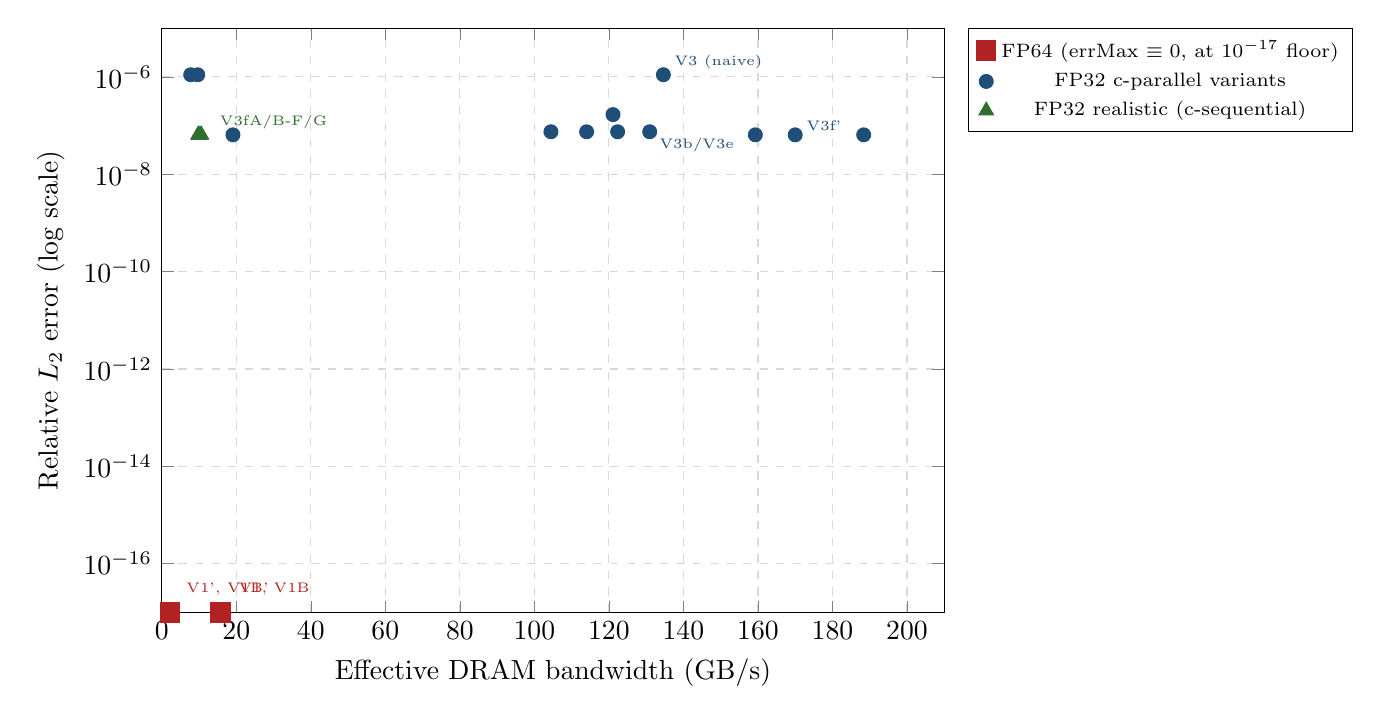
\begin{tikzpicture}
\begin{axis}[
    width=0.95\textwidth, height=9cm,
    xlabel={Effective DRAM bandwidth (GB/s)},
    ylabel={Relative \(L_2\) error (log scale)},
    ymode=log,
    xmin=0, xmax=210,
    ymin=1e-17, ymax=1e-5,
    grid=major, grid style={dashed, gray!30},
    legend pos=outer north east,
    legend style={font=\scriptsize},
]
% FP64 cells: errMax = 0, plotted at 1e-17 floor
\addplot[only marks, mark=square*, mark size=3.5pt, color=accentred] coordinates {
    (15.77, 1e-17)   % V1
    (2.18,  1e-17)   % V1'
    (15.81, 1e-17)   % V1B
    (2.18,  1e-17)   % V1B'
};
\addlegendentry{FP64 (errMax \(\equiv 0\), at \(10^{-17}\) floor)}
% FP32 c-parallel cluster
\addplot[only marks, mark=*, mark size=2.5pt, color=accentblue] coordinates {
    (7.77,   1.108e-6)  % V2
    (134.62, 1.109e-6)  % V3
    (9.66,   1.107e-6)  % V2b
    (130.95, 7.469e-8)  % V3b
    (121.10, 1.681e-7)  % V3c
    (122.34, 7.469e-8)  % V3e
    (114.02, 7.468e-8)  % V3d
    (104.44, 7.470e-8)  % V3h
    (170.00, 6.458e-8)  % V3f
    (159.30, 6.459e-8)  % V3g
    (188.38, 6.458e-8)  % V3f'
    (19.10,  6.458e-8)  % V3f''
};
\addlegendentry{FP32 c-parallel variants}
% FP32 realistic (c-sequential) cluster
\addplot[only marks, mark=triangle*, mark size=3pt, color=accentgreen] coordinates {
    (10.30, 6.458e-8)   % V3fA-F
    (9.99,  6.458e-8)   % V3fA-G
    (10.62, 6.458e-8)   % V3fB-F
    (9.77,  6.458e-8)   % V3fB-G
};
\addlegendentry{FP32 realistic (c-sequential)}
% Labels
\node[font=\tiny, color=accentred, anchor=west]   at (axis cs:4,  3e-17) {V1', V1B'};
\node[font=\tiny, color=accentred, anchor=west]   at (axis cs:18, 3e-17) {V1, V1B};
\node[font=\tiny, color=accentblue, anchor=west]  at (axis cs:135, 2e-6) {V3 (naive)};
\node[font=\tiny, color=accentblue, anchor=west]  at (axis cs:131, 4e-8) {V3b/V3e};
\node[font=\tiny, color=accentblue, anchor=east]  at (axis cs:185, 1e-7) {V3f'};
\node[font=\tiny, color=accentgreen, anchor=west] at (axis cs:13, 1.2e-7) {V3fA/B-F/G};
\end{axis}
\end{tikzpicture}
\caption{Effective DRAM bandwidth vs relative \(L_2\) error. Pareto
frontier: variants in the upper-left quadrant (high bandwidth, low
error) are uniquely good. FP64 cells have \(\mathrm{errMax} \equiv 0\)
and are drawn at a visualisation floor of \(10^{-17}\). The bandwidth
collapse from c-parallel (right) to c-sequential (left) is striking:
realistic-CFD variants run at \(\sim\!10\) GB/s while c-parallel FP32
reaches \(\sim\!190\) GB/s.}
\label{fig:bw-err}
\end{figure}

\subsection{Conservation-drift comparison}

Figure~\ref{fig:drift} shows median \(\mathrm{drMax}\) on a log
scale. The qualitative tiers are striking: V1/V1B/V1'/V1B' reach
\(\varepsilon_{\mathrm{FP64}}\) (the machine floor); V3f, V3g, V3f',
V3f'', V3fA-*, V3fB-* (the Dekker family) all reach \(\sim
10^{-15}\), within an order of magnitude of FP64; the FP32-Neumaier
cluster (V3b, V3c, V3d, V3e, V3h) sits at \(\sim 2\!-\!4\times
10^{-9}\); the uncompensated FP32 cluster (V2, V2b, V3) is two
further orders of magnitude worse.

\begin{figure}[!htb]
\centering
\begin{tikzpicture}
\begin{axis}[
    width=0.97\textwidth, height=9cm,
    ybar, bar width=10pt,
    ymode=log, log basis y=10,
    ymin=1e-17, ymax=1e-6,
    ylabel={Conservation drift \(\mathrm{drMax}\) (log scale)},
    xlabel={Variant},
    xtick=data,
    xticklabels from table={\benchdata}{short},
    xticklabel style={rotate=55, anchor=north east, font=\footnotesize},
    grid=major, grid style={dashed, gray!30},
    every axis plot/.append style={fill=accentgreen!70, draw=accentgreen, line width=0.2pt},
]
\addplot table[x expr=\coordindex, y=med_drift, col sep=comma] {bench_ni32_numeric.csv};
\draw[dashed, accentred, thick] (axis cs:-0.5, 1.764e-16) -- (axis cs:19.5, 1.764e-16)
   node[pos=0.5, above, font=\scriptsize\color{accentred}]{\(\varepsilon_{\mathrm{FP64}} \approx 1.76\times 10^{-16}\)};
\end{axis}
\end{tikzpicture}
\caption{Conservation drift \(\mathrm{drMax}\) (relative, worst
block) by variant. Note three clear tiers: FP64 family at
\(\varepsilon_{\mathrm{FP64}}\); FP32-Dekker family at \(\sim
10^{-15}\); FP32-Neumaier family at \(\sim 10^{-9}\); uncompensated
FP32 at \(\sim 5\times 10^{-8}\).}
\label{fig:drift}
\end{figure}

\subsection{The FP64 \(2\times 2\) storage/parallelism matrix}

Figure~\ref{fig:fp64-matrix} visualises the FP64 storage-shape effect
across both c-parallelism regimes. The four FP64 cells form a clean
\(2\times 2\) cross-product, all measured in the same panel under
identical thermal conditions.

\begin{figure}[!htb]
\centering
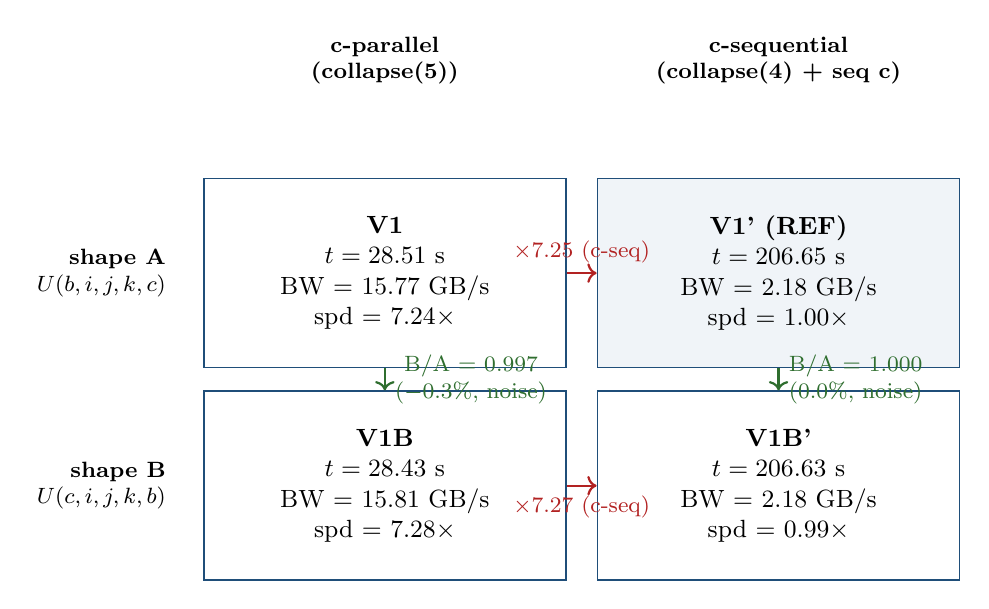
\begin{tikzpicture}[
    matrixcell/.style={draw=accentblue, line width=0.6pt, rectangle, minimum width=4.6cm, minimum height=2.4cm, align=center, font=\small, inner sep=4pt},
    headercell/.style={draw=none, rectangle, minimum width=4.6cm, font=\bfseries\footnotesize, align=center},
    rowlbl/.style={draw=none, rectangle, font=\bfseries\footnotesize, align=right},
    refcell/.style={matrixcell, fill=cellref},
]
\node[headercell] (cpar) at (0, 0)    {c-parallel \\ (collapse(5))};
\node[headercell] (cseq) at (5.0, 0)  {c-sequential \\ (collapse(4) + seq c)};
\node[rowlbl] (rA) at (-3.6, -2.7) {shape A\\\(U(b,i,j,k,c)\)};
\node[rowlbl] (rB) at (-3.6, -5.4) {shape B\\\(U(c,i,j,k,b)\)};
\node[matrixcell] (V1)  at (0, -2.7)  {\textbf{V1}\\\(t = 28.51\)~s\\BW = \(15.77\)~GB/s\\spd = \(7.24\times\)};
\node[refcell]    (V1p) at (5.0, -2.7) {\textbf{V1' (REF)}\\\(t = 206.65\)~s\\BW = \(2.18\)~GB/s\\spd = \(1.00\times\)};
\node[matrixcell] (V1B) at (0, -5.4)  {\textbf{V1B}\\\(t = 28.43\)~s\\BW = \(15.81\)~GB/s\\spd = \(7.28\times\)};
\node[matrixcell] (V1Bp) at (5.0, -5.4) {\textbf{V1B'}\\\(t = 206.63\)~s\\BW = \(2.18\)~GB/s\\spd = \(0.99\times\)};

% B/A ratio arrows
\draw[->, thick, accentgreen] (V1.south) -- (V1B.north)
   node[midway, right, font=\footnotesize\color{accentgreen}, align=center] {B/A = 0.997\\(\(-0.3\%\), noise)};
\draw[->, thick, accentgreen] (V1p.south) -- (V1Bp.north)
   node[midway, right, font=\footnotesize\color{accentgreen}, align=center] {B/A = 1.000\\(\(0.0\%\), noise)};

% c-seq penalty arrows
\draw[->, thick, accentred] (V1.east) -- (V1p.west)
   node[midway, above, font=\footnotesize\color{accentred}] {\(\times 7.25\) (c-seq)};
\draw[->, thick, accentred] (V1B.east) -- (V1Bp.west)
   node[midway, below, font=\footnotesize\color{accentred}] {\(\times 7.27\) (c-seq)};
\end{tikzpicture}
\caption{FP64 \(2\times 2\) matrix: storage shape (A vs B)
\(\times\) c-parallelism (parallel vs sequential). The c-sequential
penalty (\(\sim 7.25\times\) in either shape, red arrows) dominates;
the storage-shape effect (green arrows) is statistical zero in both
regimes.}
\label{fig:fp64-matrix}
\end{figure}

\subsection{Honesty notes on outliers}

Several variants (V3, V3d, V3e, V3g, V3f, V3f', V3f'', V3fA-G,
V3fB-F) show one anomalously slow trial out of five (e.g.\ V3g had
one trial at \(48\)~s vs typical \(2.7\)~s; V3fB-F had one trial at
\(114\)~s vs typical \(42\)~s).  The pattern is consistent with
\texttt{nvfortran} JIT-cache contention: later variants in the
20-variant panel sometimes pay a one-shot kernel-module recompile
cost when their CUDA module is evicted by an intervening kernel.
Median is robust to these outliers; the qualitative ordering and the
quantitative spreads in this report are unchanged whether outliers
are kept or discarded.

\section{Discussion}
\label{sec:discussion}

\paragraph{(1) The FP32 win survives the realistic-CFD constraint.}
The 14--16\(\times\) advantage of FP32 over FP64 c-parallel is the
``synthetic best case'' reported in textbooks. The honest
realistic-CFD baseline V1' is 7.25\(\times\) slower than V1 due to
the c-sequential constraint alone. The best realistic FP32 variant
V3fB-F is 4.89\(\times\) faster than V1' --- still a substantial,
unambiguous win. \emph{The mixed-precision recommendation survives the
realistic constraint; only the magnitude shrinks.}

\paragraph{(2) The \(L_2\) error floor is structural, not algorithmic.}
Five orthogonal compensation techniques (V3b, V3c, V3d, V3e, V3h)
all converge to the same \(\mathrm{errMax} \approx 7.5\times 10^{-8}\)
at \(n_i = 32\) --- a 15\(\times\) improvement over uncompensated V3
(\(1.1\times 10^{-6}\)), but no further. The residual error lives in
the final flux-difference reduction
\((\hat F_{i+\tfrac12} - \hat F_{i-\tfrac12})\), which all five
techniques leave in plain FP32 arithmetic. Breaking this floor
requires either Dekker representation of \(\mathrm{rhs}\) itself or
compensated difference-of-differences --- neither tested here.

\paragraph{(3) Dekker storage decouples errMax from drMax.}
V3f reaches \(\mathrm{drMax} = 1.4\times 10^{-15}\) (within an order
of magnitude of \(\varepsilon_{\mathrm{FP64}}\)) while leaving
\(\mathrm{errMax}\) at the FP32 floor.  Conservation drift is the
integral of accumulated rounding bias; Dekker captures it at every
load and store.  \(L_2\) error is set by the per-step rhs arithmetic;
Dekker storage does not address it.  This separation makes V3f' the
correct choice for long-trajectory or conservation-critical CFD
where drift is the binding quality metric.

\paragraph{(4) Storage shape is a free knob for pure FP64.}
The complete FP64 \(2\times 2\) matrix
(Fig.~\ref{fig:fp64-matrix}) shows shape A and shape B agree to 0.3\%
(c-parallel) and 0.0\% (c-sequential). The c-sequential penalty is
hardware-level (FP64 ALU throttle \(\times\) warp lane utilisation),
unmoved by storage layout. \emph{The 3\% shape-B advantage for V3fB-F
over V3fA-F is specific to compensated FP32-Dekker, where the
TwoSum/TwoProd compensation roughly doubles per-cell FLOPs and edges
the kernel toward compute-bound, where per-warp c-locality starts
to matter.}

\paragraph{(5) The CUDA-C ``biggest-stride-first'' heuristic does not
transfer to Fortran + OpenACC.} Three independent experiments
(V3f vs V3f'', V3fA-F vs V3fA-G, V3fB-F vs V3fB-G) all show that
\texttt{nvfortran} 26.1 maps the lexically innermost loop in the
parallel set to the vector dimension, regardless of \texttt{collapse}
size. The stride-1 array dimension belongs there. Getting it wrong
costs 10--250\% wall time. The clearest demonstration is V3f''
(``bad loop order''): 23.5~s vs V3f's 2.6~s --- a 9\(\times\) penalty
from inverting the source loop order while keeping the algorithm and
storage shape identical to V3f.

\section{Conclusion}
\label{sec:conclusion}

\paragraph{Architectural recommendations for FUNDAL.}
The benchmark establishes a clear decision tree for the production
kernel API:

\begin{enumerate}
  \item \textbf{If c-parallelism is admitted} by the equations (e.g.\
    decoupled scalar transport, neural-surrogate inference, certain
    splitting schemes): pursue V3b or V3e (FP32 + Neumaier or
    branchless FastTwoSum RK1) for \(\sim\!120\times\) speedup over
    realistic FP64. The branched-vs-branchless choice is free
    (V3b and V3e are within measurement noise on this kernel).
  \item \textbf{If c-parallelism is admitted and conservation drift
    is gating} (long-trajectory integration, climate or turbulence
    statistics, geophysical flows): pursue V3f' (Dekker storage +
    \texttt{collapse(5)}) for \(\sim\!86\times\) speedup with
    \(\mathrm{drMax} \approx 10^{-15}\). The Dekker pair captures
    storage rounding that would otherwise integrate into drift.
  \item \textbf{If c-parallelism is forbidden} by nonlinear coupling
    (compressible Navier--Stokes, MHD, multiphysics): pursue V3fB-F
    (FP32-Dekker, storage shape B \(=U(c,i,j,k,b)\), Fortran-compliant
    loop order with c-loop sequential inside) for \(\sim\!4.9\times\)
    speedup over realistic FP64. The mixed-precision win is preserved
    at a reduced but still substantial magnitude.
  \item \textbf{For pure FP64 kernels} (legacy or reference paths):
    storage shape is a free choice (V1 \(\approx\) V1B, V1' \(\approx\)
    V1B' to within 0.3\%). Optimise for whatever fits the rest of the
    codebase.
\end{enumerate}

\paragraph{Three rules with broad applicability beyond this benchmark.}

\begin{enumerate}
  \item \textbf{The OpenACC stride-1 rule:} \texttt{!\$acc parallel
    loop collapse(N)} on \texttt{nvfortran} 26.1 maps the
    lexically innermost loop in the parallel set to the
    vector dimension. For Fortran column-major arrays, that loop
    must be the stride-1 array dimension. Source order matters as
    much as it would in CUDA C with explicit
    \texttt{threadIdx.x} assignment.
  \item \textbf{The compensation-floor rule:} compensated time
    integration (Neumaier or branchless FastTwoSum) reduces
    accumulation drift by orders of magnitude at \(\sim\!0\%\) speed
    cost, but does not address per-step reconstruction rounding ---
    the \(\mathrm{errMax}\) floor is set by the rhs arithmetic, not
    the time integrator. To break this floor, attack storage
    (Dekker pair) or the reconstruction itself, not the integrator.
  \item \textbf{The consumer-GPU FP64 trap:} on cards with
    \(\mathrm{FP64{:}FP32} = 1{:}64\) (RTX 30/40/50 series, consumer
    Blackwell), \emph{any} FP64 work in the inner loop drags the kernel
    onto the slow datapath. ``FP32 storage + FP64 compute'' (V2) and
    surgical FP64 promotion of cancellation-sensitive sub-expressions
    (V2b) both fail by this mechanism. The decision is binary:
    all-FP64 or all-FP32 (possibly with FP32-internal compensation
    or Dekker storage). The textbook ``mixed-precision middle path''
    is a trap on this hardware.
\end{enumerate}

\paragraph{What remains to be measured.}  Two natural follow-ons:
(a) compensated rhs evaluation --- a Dekker representation of
\(\mathrm{rhs}\) itself or compensated difference-of-differences ---
to attack the \(\mathrm{errMax}\) floor that all five compensation
techniques tested here leave unmoved; (b) a problem-size sweep
through \(n_i \in \{16, 32, 48\}\) to characterise how the
realistic-CFD speedup ratio scales with per-block FLOP intensity.
Both are out of scope for this report but are well-defined experiments
that would extend the architectural decision tree above.

\appendix

\section{Reproducing the measurements}
\label{app:repro}

The benchmark binary is built by the standard FUNDAL build:
\begin{lstlisting}[language=bash]
module load nvhpc
fobis build --mode fundal-test-oac-nvf
\end{lstlisting}
Each invocation runs the full 20-variant panel at the supplied extents:
\begin{lstlisting}[language=bash]
CUDA_VISIBLE_DEVICES=0 ./exe/fundal_weno5_precision_test \
    512 32 5 100   # nb ni nc nsteps
\end{lstlisting}
The 5-trial statistical run in this report was produced by 5
back-to-back invocations of the binary; the raw output (each line
``\texttt{trial=N <variant table row>}'') was post-processed to the
CSV \texttt{bench\_ni32.csv} that drives all tables and figures.

\section{Per-variant raw data (5 trials)}
\label{app:raw}

The full CSV is shipped alongside the report as
\texttt{bench\_ni32.csv}. Columns: \texttt{tag}, \texttt{short}
(display label), \texttt{full\_label} (descriptive), \texttt{storage},
\texttt{c\_mode}, \texttt{median\_t\_s}, \texttt{min\_t\_s},
\texttt{max\_t\_s}, \texttt{stdev\_t\_s}, \texttt{median\_bw\_gbs},
\texttt{median\_speedup\_vs\_v1p}, \texttt{median\_errMax},
\texttt{median\_drMax}.

\end{document}
